\chapter{Hyperparameter optimisation of a classifying neural network}
\label{chp:simpleNN}

The adversarial neural network is based on a common classifying neural network, which is trained on signal/background separation. The output of that classifier is then used as input for the adversary to create a negative feedback for the classifier.
Before the adversarial, second network is added, the classifying network is optimised on its own to ensure that its setup is sufficient for the classification task.
During the adversarial training, this setup can be updated if the structure is not optimised for the additional task of a model that is less sensitive to systematic uncertainties.

This chapter describes the hyper-parameter optimisation of the first network starting with the motivation of the input information.
The second section explains the choice of the architecture followed by the step-wise setup of the optimiser.
Lastly regularisation of the network is tested and described.
The overall aim of the description is to provide some understanding on the hyper-parameters available and their correlations. The impact of the hyper-parameters on the training results is presented not only to introduce their function but also to motivate possible solutions later on.

To train the network and test its performance, all its parts need to be in place. Therefore, all hyper-parameters had to be initialized with values assumed to represent a reliable setup. Initially, this was accomplished by starting with a very simple network using a minimal set of hyper-parameters which were then developed to a more and more optimised network. The results shown in this work are going to be based on the final choice of hyper-parameters, where only one parameter is then varied at a time to explain the impact of a particular tuning. Sometimes, this leads to the effects of a hyper-parameter to be less powerful. The already optimised model is relatively stable, and, if no significant impact is visible, the plots are not shown. For that reason, section~\ref{sec:simplesetup} will already introduce the final network structure, which is then explained and motivated step by step.

The structure was achieved within reason and the computational power constraints. There certainly are hyper-parameters that deserve more attention, and in addition to that, there are alternative setups for the whole network that were not tested. A further investigation of network optimisation is, without a doubt, very promising.


\section{Technical details}
\label{sec:technicals}

The artificial neural networks in this thesis were created using the Keras python library~\cite{chollet2015keras}.
Keras is an application programming interface written in python and able to run on Tensorflow~\cite{tensorflow2015-whitepaper}, CNTK~\cite{cntk} or Theano~\cite{theano}. It was developed by google and summarises the necessary calculations for running a deep neural network training in fast and easy modules.
The backend is the package responsible for the underlying vector calculations needed for the network setup and training. In this work, the Tensorflow package was used as a backend.

\section{Final setup of the network}
\label{sec:simplesetup}

This section describes the fully optimised classifier which is then, parameter-wise, varied during this chapter to motivate the final network structure.
The hyperparamters are listed and the loss curve, the ROC curve, and the final separation are shown in figure~\ref{fig:simple:final}. They are the main tools a training performance is evaluated on in this thesis. For the sake of completeness, the agreement between nominal and systematic response is also shown as it will be a standard inclusion for the plots during the adversarial training.


\begin{itemize}
\item Input: \num{14} variables motivated by a BDT variable scan~\cite{Finelli:2667560}.
\item Hidden layers: \num{6} \ELU layers $\times$ \num{128} nodes each
\item Output layer: \num{1} \SIGMOID node
\item Optimisation: SGD, Learning rate $=0.06$, momentum $=0.3$, no nesterov, no decay
\item Duration: 600 epochs
\end{itemize}

\begin{figure}[htbp]
    \centering
    \begin{subfigure}[b]{0.48\textwidth}
        \includegraphics[width=\textwidth]{standard_separation}
        \caption{}
        \label{fig:simple:final:sepa}
    \end{subfigure}
\quad
    \begin{subfigure}[b]{0.48\textwidth}
        \includegraphics[width=\textwidth]{standard_syst}
        \caption{}
        \label{fig:simple:final:syst}
    \end{subfigure}

    \begin{subfigure}[b]{0.48\textwidth}
		\includegraphics[width=\textwidth]{standard_ROC}
		\caption{}
		\label{fig:simple:final:roc}
	\end{subfigure}
\quad
	\begin{subfigure}[b]{0.48\textwidth}
		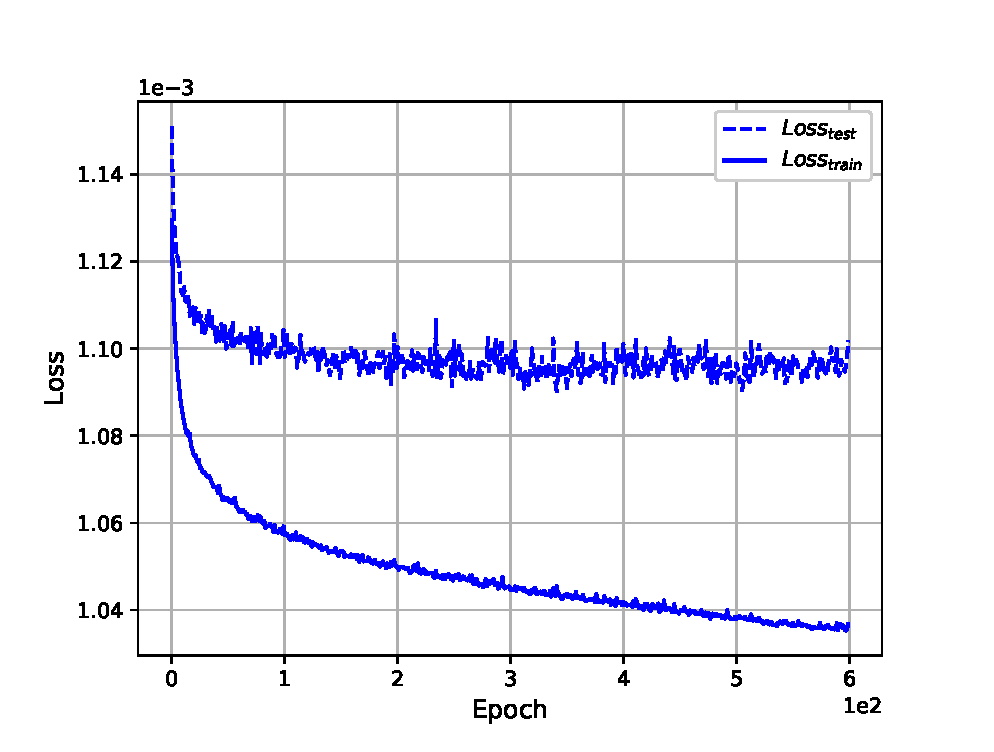
\includegraphics[width=\textwidth]{standard_losses}
		\caption{}
		\label{fig:simple:final:loss}
	\end{subfigure}
    \caption[Network performance of the classifier]{Figure~\subref{fig:simple:final:sepa} shows the response of the classifier. The solid lines represent the training sample and the dashed lines the test sample. Figure~\subref{fig:simple:final:syst} shows the difference for response in systematic and nominal samples. The solid lines represent the nominal samples and the dashed line the systematic sample. Figure~\subref{fig:simple:final:roc} shows the ROC curve. The dashed line is the training curve and the solid line is the test curve. Figure~\subref{fig:simple:final:loss} diagrams the losses with dashed for test and solid for training.}
	\label{fig:simple:final}
\end{figure}


\section{The input variables}

Two sets of input variables were tested for the classifier.
The first one is a set of simple kinematic variables. This is tested to exploit a neural network's ability to deduce all further information from the complete basis of a system.
The second set of variables uses more complex variables based on the most significant variables for a boosted decision tree usage on a similar problem.
The variable sets used were:
%
%
%
\begin{table}[h]
    \begin{minipage}{.5\linewidth}
      \centering
		\begin{tabular}{l}
		Variable         \\ \hline
		\pTmiss          \\ \hline
		$|\eta_{jet1}|$  \\ \hline
		$|\eta_{jet1}|$  \\ \hline
		$|\eta_{lep1}|$  \\ \hline
		$|\eta_{lep2}|$  \\ \hline
		${\pT}_{jet1}$   \\ \hline
		${\pT}_{jet2}$   \\ \hline
		${\pT}_{lep1}$   \\ \hline
		${\pT}_{lep2}$   \\ \hline
		$\phi_{jet1}$    \\ \hline
		$\phi_{jet2}$    \\ \hline
		$\phi_{lep1}$    \\ \hline
		$\phi_{lep2}$    \\ \hline
		\end{tabular}
		\caption{Simple kinematic variables}
    \end{minipage}%
    \begin{minipage}{.5\linewidth}
      \centering
		\begin{tabular}{l}
		Variable                   \\ \hline
		$m_{lep1} + m_{jet2}$      \\ \hline
		${\pT}_{lep1} + {\pT}_{lep2} + \pTmiss     $     \\ \hline
		${\pT}_{jet1} + {\pT}_{jet2}    $     \\ \hline
		$m_{lep1} + m_{jet1}$      \\ \hline
		${\pT}_{lep1} - {\pT}_{jet1}$\\ \hline
		${R}_{lep1} - {R}_{jet2}$    \\ \hline
		$R_{lep1, lep2} - R_{jet2}$       \\ \hline
		$m_{lep2} + m_{jet1}$        \\ \hline
		${\pT}_{jet2}$               \\ \hline
		${R}_{lep1} - {R}_{jet1}$	 \\ \hline
		${R}_{lep1} - {R}_{jet1}$	 \\ \hline
		${R}_{lep2} - {R}_{jet2}$	 \\ \hline
		$\text{Centrality}_{lep2} + \text{Centrality}_{jet2}$ \\ \hline
		${R}_{lep2} - {R}_{jet1}$    \\ \hline
		\end{tabular}
		\caption{Complex variables}
    \end{minipage} 
\end{table}
%
Figure \ref{fig:vars} shows a comparison of the separation and the loss curves for both variable sets. It is visible that for the set of simple variables the network runs into overtraining after about \num{200} epochs visible in plot~\ref{fig:vars:simple:loss} because \losstrain and \losstest start to diverge. This also results in a bad separation with a strong disagreement between the two samples. One way overtraining could be avoided using simple kinematic variables would be to stop earlier; in this case after about 200 epochs. There is an argument for testing a simple set of variables for a shorter training duration. However, this optimisation process would be a project of its own because all the other parameter would have to be optimised accordingly. Furthermore, in this work one has to keep in mind that the network is supposed to be used in adversarial setup later. This demands for a longer training period and a large number of features, with a strong separating potential, to be available. Otherwise the probability of finding a classifier, less sensitive to a systematic uncertainty, decreases and the behaviour of the losses has to supervised very carefully.

Showing an overall good performance, the set of complex variables, as suggested by the boosted decision tree variable scan, performed in the analysis \enquote{Measurement of the cross-section for the production of a \PW boson in association with a top quark at \SI{13}{\tera \electronvolt}} was chosen~\cite{Finelli:2667560}. Please note that the set of variables in the paper referred to does not always agree because the set used in this work was just inspired by it.

\begin{figure}[htbp]
    \centering
    \begin{subfigure}[b]{0.45\textwidth}
        \includegraphics[width=\textwidth]{standard_separation}
        \caption{}
        \label{fig:vars:standard:sep}
    \end{subfigure}
\quad
    \begin{subfigure}[b]{0.45\textwidth}
        \includegraphics[width=\textwidth]{simple_vars_separation}
        \caption{}
        \label{fig:vars:simple:sep}
    \end{subfigure}

    \begin{subfigure}[b]{0.45\textwidth}
		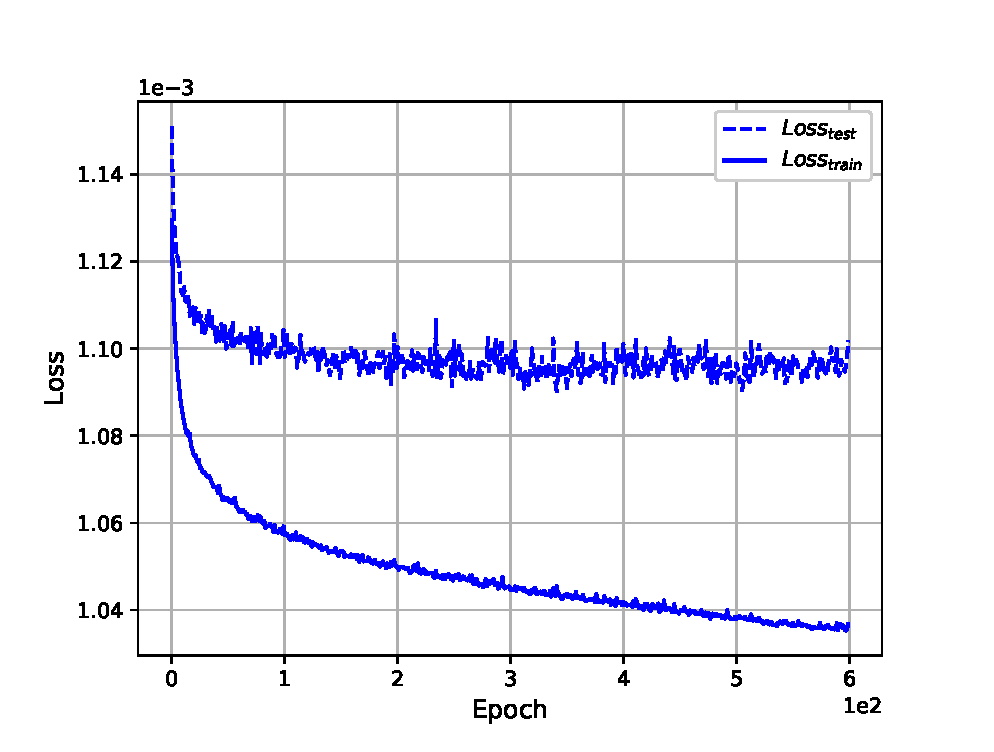
\includegraphics[width=\textwidth]{standard_losses}
		\caption{}
		\label{fig:vars:standard:loss}
	\end{subfigure}
\quad
	\begin{subfigure}[b]{0.45\textwidth}
		\includegraphics[width=\textwidth]{simple_vars_losses}
		\caption{}
		\label{fig:vars:simple:loss}
	\end{subfigure}
    \caption[Performance of the classifier using different variables]{Figure~\subref{fig:vars:standard:sep} and figure~\subref{fig:vars:simple:sep} show the separation for the complex and simple variables respectively. The losses for the variable sets are depicted in figure~\subref{fig:vars:standard:loss} and figure~\subref{fig:vars:simple:loss}.}
	\label{fig:vars}
\end{figure}





\section{The network architecture}

The architecture of the neural network is formed by its nodes and layers. The choice of the architecture is nontrivial and, as a lot of aspects of machine learning, not an exact science.
However, one can make some assumptions about the appropriate architecture.
First of all, the complexity of the model should about match the complexity of the task assigned. Although it usually is not trivial to find an estimator for a task's complexity and even less to match it to a certain architecture, a test series often leads to a good estimate. Another possible starting point is the amount of variables necessary to fully describe a system resulting in the minimum variable number necessary to input in the network. This also gives a first estimate on how large the architecture should at least be.
Both the depth and the overall size of the model play a role. A simplified way of explaining these two properties is by saying that the depth defines how often the input is processed while the number of nodes is the number of features that can be kept during each step of processing.

In general, an architecture that is too deep and wide would learn training set related features too fast, meaning it overtrains before it finds a good minimum. This can be seen in an early divergence between the training loss and the test loss. An architecture too simple is not able to pick up the features of the task at all resulting in no learning. In other words, the loss stays constant or changes very slowly.

In this work, a test-series was performed. The network was trained for a wide range of combinations of nodes and layers; $\text{nodes}\in[8,512]$ and $\text{layers}\in[1,10]$. For the sake of simplicity, the number of nodes per layer was kept constant during each training. Two variables were then plotted against the size of the architecture. First, the overall smallest loss the model achieved during the training was plotted. The other variable was the minimal difference between the training and the test loss. To keep it simple the complexity of the architecture was defined as the product of nodes and layers. These are certainly not the most sophisticated indicators for the model's complexity and its performance. However, the plots do allow for educated guesses for a good choice of architecture.

Figure~\ref{fig:minimal_loss} shows that more complex architectures also achieve smaller loss values.
This, unfortunately is not a clear estimator for overall performance since heavily overtrained networks will achieve low loss values as well.
Therefore, a second estimator was taken into account. Figure~\ref{fig:minimal_diff} shows the minimal difference between \losstrain and \losstest achieved during the whole training process.
There are two regions showing the minimum difference. The first region includes simple architectures.
This, however, is a result of a slow learning process. In this case, the respective overall loss is not minimal and the network's separation power is very low.
The second region, with a complexity of \numrange{500}{800}, was used as the region of choice; before heavy overtraining occurs.
As a result, a more complex architecture in this region, comprising \num{6} layers with \num{128} nodes each, was chosen.
Although this choice seems fairly arbitrary at this point, there is arguments for a complex architecture as it can always be regulated using dropout if need be. Additional prove that further increasing the architecture leads to overtraining can be seen in the loss for a complex architecture in figure~\ref{fig:complex_arch}. Here the overtraining becomes visible in the difference between the two curves and their overall odd behaviour. Here the two loss functions are not only diverging but the test loss also shows non-linear behaviour around \num{400} epochs. This is usually not expected because once a feature only relevant for the training set has been included it stays problematic.



\begin{figure}[htbp]
    \centering
    \begin{subfigure}[b]{0.45\textwidth}
        \centering
        \includegraphics[width=\textwidth]{figures_simpleNN/minimal_loss.eps}
        \caption{Minimal loss}
        \label{fig:minimal_loss}
    \end{subfigure}%
\quad
    \begin{subfigure}[b]{0.45\textwidth}
        \centering
        \includegraphics[width=\textwidth]{figures_simpleNN/minimal_diff.eps}
        \caption{Minimal loss difference}
        \label{fig:minimal_diff}
    \end{subfigure}
    \caption[Network performance's dependency on the architecture]{Figure~\subref{fig:minimal_loss} shows the minimal overall loss achieved during the training for the range of architectures. Figure~\subref{fig:minimal_diff} shows the minimal difference between \losstrain and \losstest achieved.}
    \label{fig:net_complexity}
\end{figure}



\begin{figure}[htbp]
	\centering
	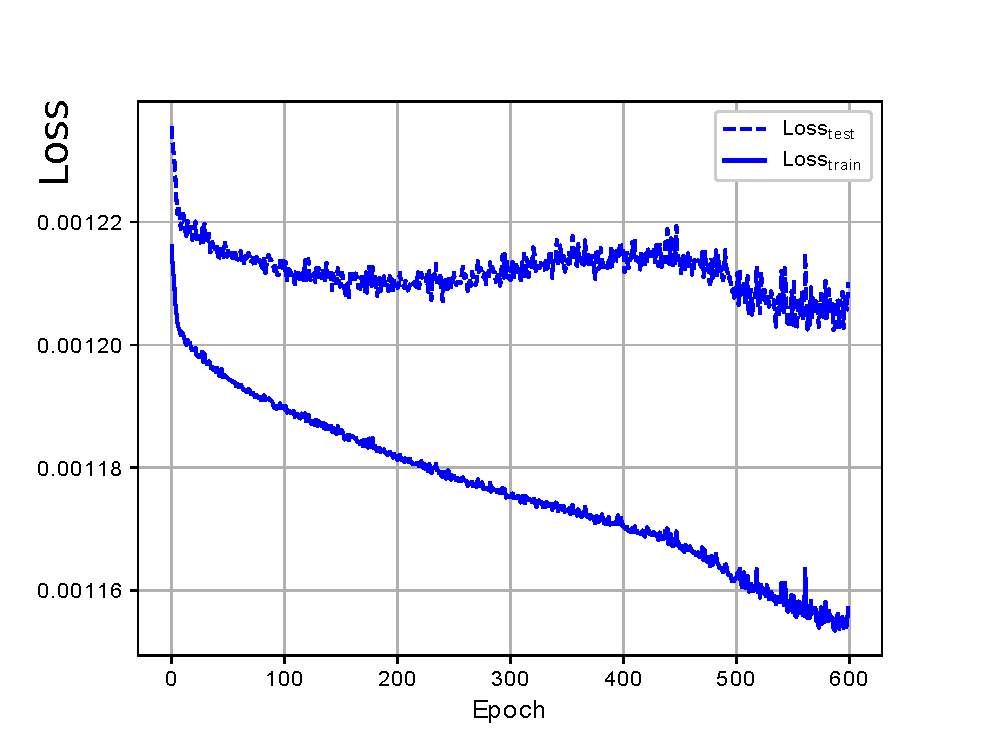
\includegraphics[width=0.8\textwidth]{complex_arch_losses}
	\caption[Classifier losses for a complex architecture]{Loss function for the classifier for \num{8} layers and \num{512} nodes each. A large disagreement between the two curves is visible which is a sign for overtraining.}
	\label{fig:complex_arch}
\end{figure}

In addition to the choice of the architecture, the activation function for the layers has to be set.
Two different activation functions are used in the neural network. The main function connects the nodes in the hidden layers while the last one converts the output to a value between \num{0} and \num{1}. For the output the sigmoid function is a natural choice because we look at two possible labels for the outcome: signal and background. Therefore, no other activations were tested.
For the hidden layers \ELU and \RELU were tested. Figure~\ref{fig:activ} shows a comparison of the ROC curve and the loss development for both activation-functions. For \RELU, a strong disagreement between training- and test-sample occurs and \ELU became the activation function of choice. Further activation-functions were not tested due to time constraints.

\begin{figure}[htbp]
    \centering
    \begin{subfigure}[b]{0.48\textwidth}
        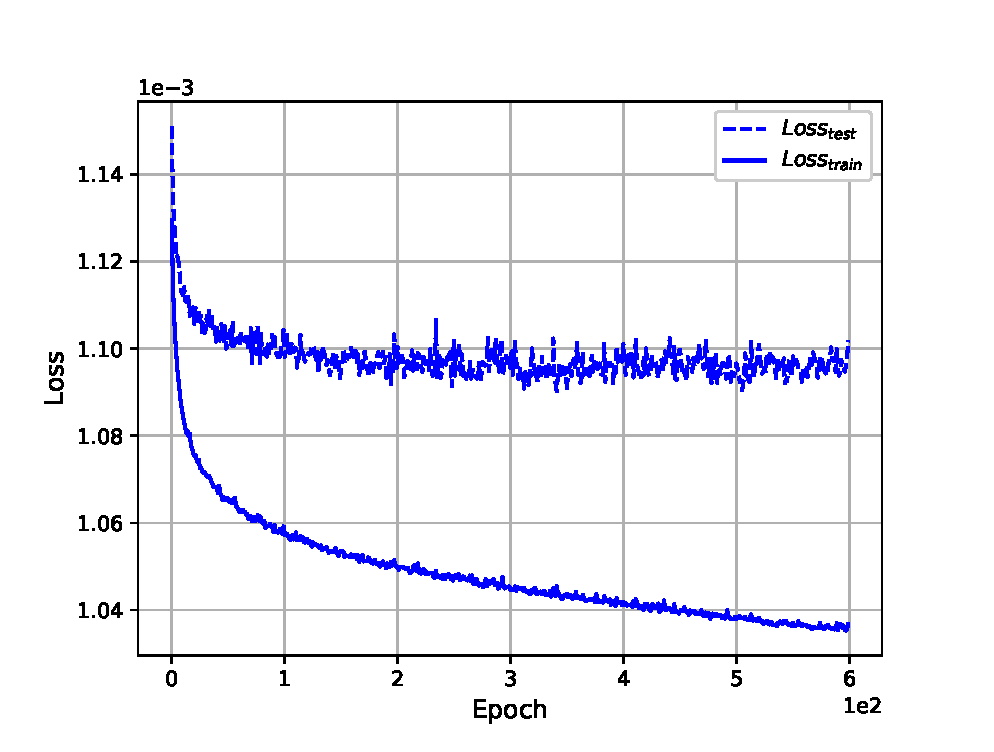
\includegraphics[width=\textwidth]{standard_losses}
        \caption{}
        \label{fig:activ:standard:loss}
    \end{subfigure}
\quad
    \begin{subfigure}[b]{0.48\textwidth}
        \includegraphics[width=\textwidth]{relu_losses}
        \caption{}
        \label{fig:activ:relu:loss}
    \end{subfigure}

    \begin{subfigure}[b]{0.48\textwidth}
		\includegraphics[width=\textwidth]{standard_ROC}
		\caption{}
		\label{fig:activ:standard:roc}
	\end{subfigure}
\quad
	\begin{subfigure}[b]{0.48\textwidth}
		\includegraphics[width=\textwidth]{relu_ROC}
		\caption{}
		\label{fig:activ:relu:roc}
	\end{subfigure}
    \caption[Classifier performance for different activation functions]{Figure~\subref{fig:activ:standard:loss} and figure~\subref{fig:activ:relu:loss} show the losses for \ELU and \RELU respectively. The ROC curves for the different activation-functions are diagrammed in figure~\subref{fig:activ:standard:roc} and figure~\subref{fig:activ:relu:roc}.}
	\label{fig:activ}
\end{figure}


\section{Setup of the optimisation}

For the most part of the optimisation, SGD was used and its tuning is shown in detail in subsection~\ref{sec:optimiser:tuning}.
Adam was also tested but not fully tuned, due to constraints on time and computational resources.
In subsection~\ref{sec:optimiser:choice}, a brief overview of the performance using Adam is given.

\subsection{Choice of the optimiser}
\label{sec:optimiser:choice}

A classic gradient-based optimiser, SGD, is compared to the adaptive optimiser, Adam. Figure~\ref{fig:opti} compares the loss development for both optimisers. It is obvious that Adam behaves strangely and it was therefore discarded. It is possible that Adam could outperform SGD for a better tuning of its hyper-parameters and it certainly is worth testing out if the computational power is provided.

\begin{figure}[htbp]
    \centering
    \begin{subfigure}[b]{0.48\textwidth}
        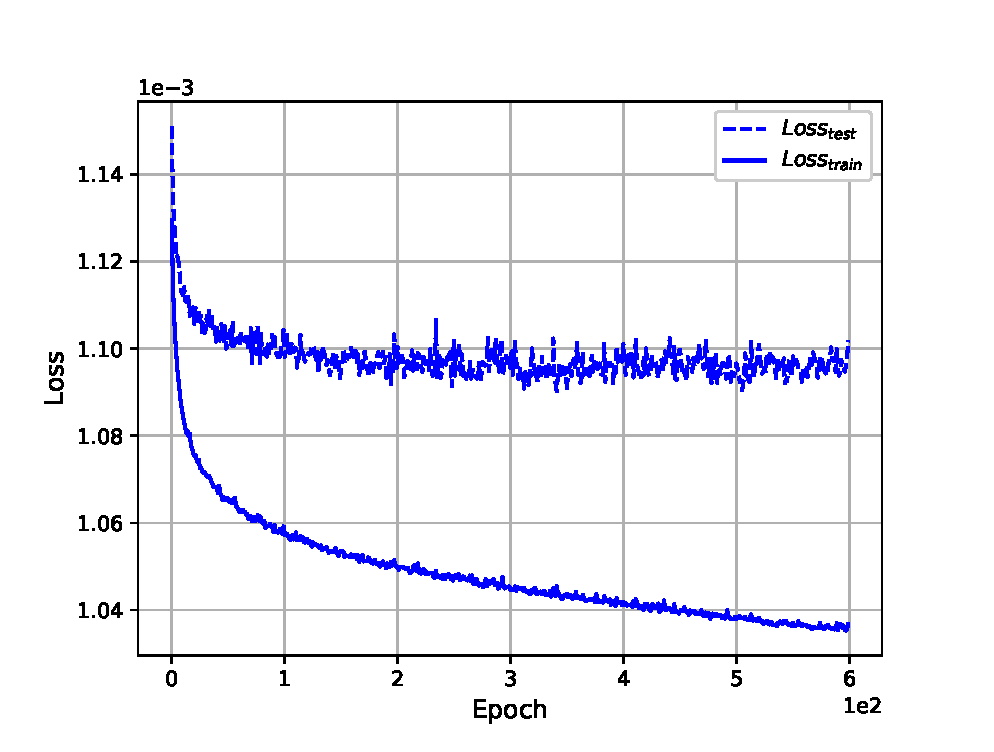
\includegraphics[width=\textwidth]{standard_losses}
        \caption{}
        \label{fig:opti:standard}
    \end{subfigure}
\quad
    \begin{subfigure}[b]{0.48\textwidth}
        \includegraphics[width=\textwidth]{adam_losses}
        \caption{}
        \label{fig:opti:adam}
    \end{subfigure}
    \caption[Classifier losses for different optimisers]{Loss curves for the chosen network architecture using SGD~\subref{fig:opti:standard} and Adam~\subref{fig:opti:adam}.}
	\label{fig:opti}
\end{figure}

\subsection{Tuning the optimiser}
\label{sec:optimiser:tuning}

As described in section~\ref{sec:optimisation}, an optimiser has several hyper-parameters of its own. In this section, the learning rate, the momentum with the option of Nesterov, and the decay parameter will be probed.
For the learning rate, a range of values between a small learning rate of \num{0.001} and high learning rates up to \num{0.5} were tested to investigate the effect on the network's ability to approach a minimum. The choice was based on how high the oscillations of the losses are and how efficiently the training converges. High learning rates were discarded for an increased probability of overtraining and a lot of unwanted oscillations while small learning rates made the training unnecessarily slow and inefficient. Figure~\ref{fig:lr} shows a comparison of the network losses for a small learning rate of \num{0.001} in subfigure~\ref{fig:lr:small} and a relatively high learning rate of \num{0.2} in subfigure~\ref{fig:lr:large}. For the small learning rate there are no signs of overtraining and no oscillations visible. However, the training converges slowly. For a high learning rate the \losstrain and \losstest show larger divergence and each curve shows more oscillations individually. In the end, an intermediate learning rate of \num{0.06} is chosen.
%
\begin{figure}[htbp]
    \centering
    \begin{subfigure}[b]{0.48\textwidth}
        \includegraphics[width=\textwidth]{smalllr_losses}
        \caption{}
        \label{fig:lr:small}
    \end{subfigure}
\quad
    \begin{subfigure}[b]{0.48\textwidth}
        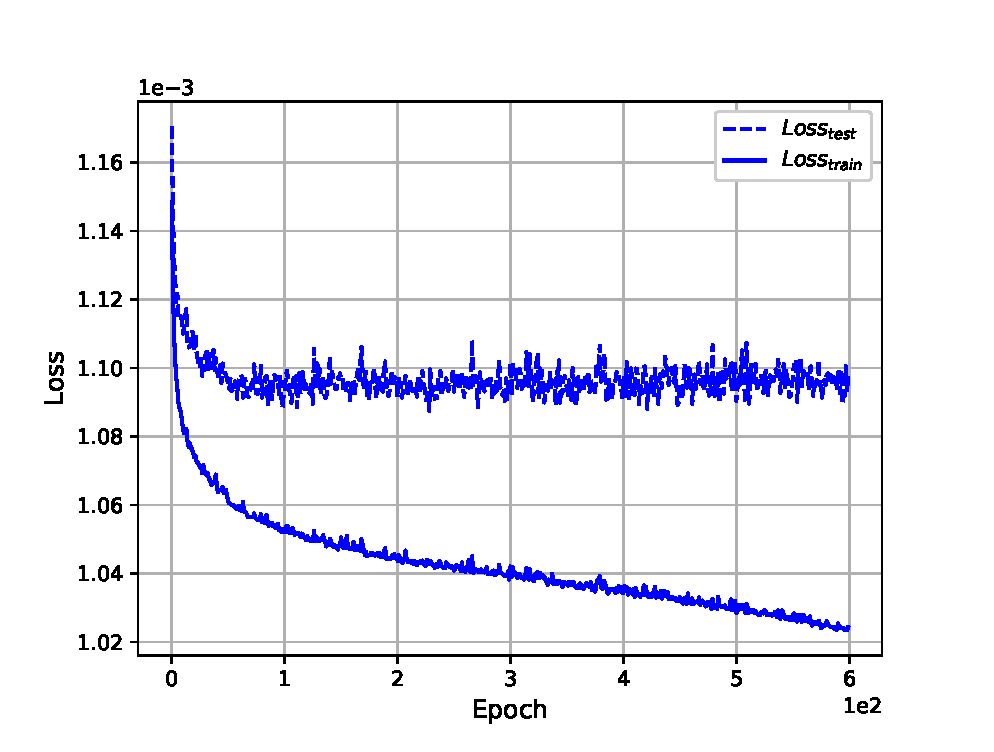
\includegraphics[width=\textwidth]{largelr_losses}
        \caption{}
        \label{fig:lr:large}
    \end{subfigure}
    \caption[Classifier loss for different learning rates]{Loss behaviour for learning rates of different scales. Figure~\subref{fig:lr:small} shows losses for \num{0.001} and figure~\subref{fig:lr:large} for~\num{0.2}.}
	\label{fig:lr}
\end{figure}
%
In this setup, dropout is used. That makes it a bit more difficult to see the clear signs of overtraining as it can be avoided for many setups. For a plot that shows this, see section~\ref{sec:simple_dropout}.

Like the learning rate, the momentum was scanned over a wide range of values. Again, the risk of overtraining and the amount of oscillations was evaluated against the overall training efficiency. This resulted in a final value of \num{0.3}. In addition, the test of using Nesterov momentum did not lead to any significant effects. It was therefore not utilized to avoid using unnecessary computational power.

The decay parameter was tested to see its effect on the loss behaviour. Figure~\ref{fig:decay} shows the standard loss behaviour compared to losses for a decay value of \num{1e-6}. When decay is used, the losses in subfigure~\ref{fig:decay:decay} become slightly more stable and plateau a bit earlier and at a greater value. Overall, no significant improvement is visible. For that reason, decay is not included in the final setup of the classifier. It was kept as an option for the later combination of the classifier and the adversary where it might help keeping the model close to the optimum while slowly updating to a model less sensitive to systematics.

\begin{figure}[htbp]
    \centering
    \begin{subfigure}[b]{0.45\textwidth}
        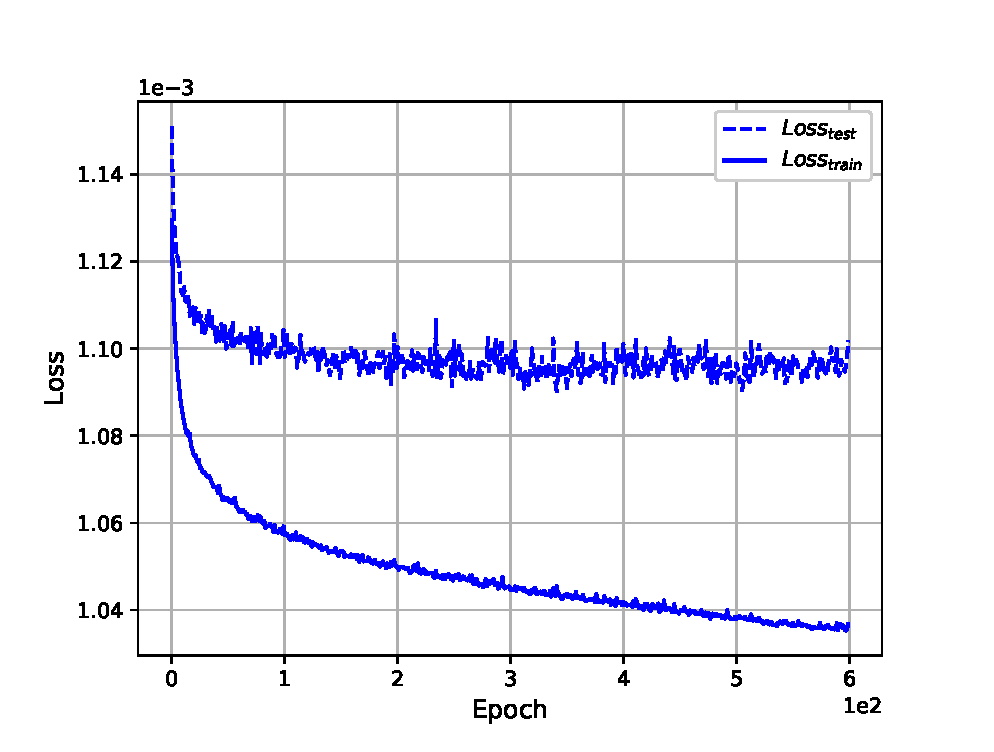
\includegraphics[width=\textwidth]{standard_losses}
        \caption{}
        \label{fig:decay:standard}
    \end{subfigure}
\quad
    \begin{subfigure}[b]{0.45\textwidth}
        \includegraphics[width=\textwidth]{decay_losses}
        \caption{}
        \label{fig:decay:decay}
    \end{subfigure}
    \caption[Performance of the classifier with decay]{Comparison of usual loss behaviour and loss behaviour including a decay paramter. Figure~\subref{fig:decay:standard} shows the losses without decay. Figure~\subref{fig:decay:decay} shows the losses for a decay parameter of \num{1e-6}}
	\label{fig:decay}
\end{figure}




\section{Regularisation}

The two regularisation tools tested were dropout-layers and batch-normalisation layers. The main purpose of dropout is regularising a network while batch-normalisation focuses on keeping all outputs on the same order which indirectly also helps the regularisation of the network.
Dropout is tested for a range of values defining the percentage of nodes turned off per iteration step. Batch-normalisation is just tested in the default setup to investigate its effects.

\subsection{Dropout}
\label{sec:simple_dropout}

A dropout layer is added to each hidden layer of the network.
Figure~\ref{fig:simple_dropout} shows the impact of dropout on the behaviour of the losses. For only \num{1} percent dropout, compared to the default \num{10} percent, overtraining occurs relatively early. For a very high dropout of \num{80} percent the losses behave strangely. The curve becomes unnaturally linear in some regions and converges less efficiently. In conclusion, dropout is a valuable addition to the network. It makes changing the architecture and the optimiser more forgiving and is a simple way to adjust a network without rearranging all hyper-parameters.

\begin{figure}[htbp]
    \centering
    \begin{subfigure}[b]{0.45\textwidth}
        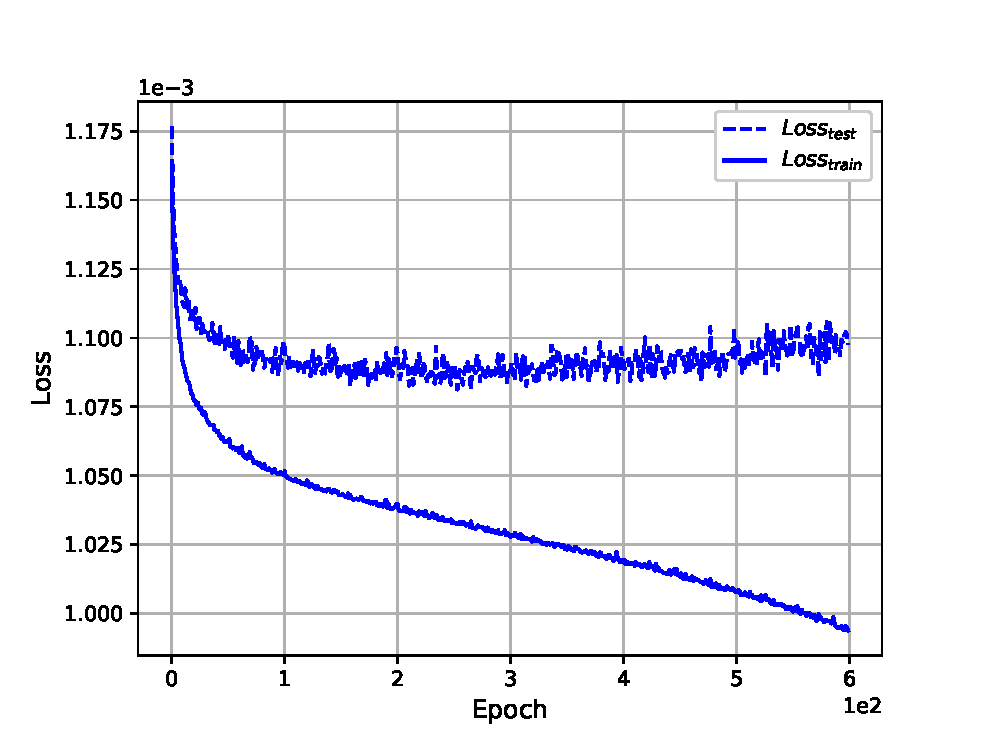
\includegraphics[width=\textwidth]{lowdrop_losses}
        \caption{}
        \label{fig:dropout:low}
    \end{subfigure}
\quad
    \begin{subfigure}[b]{0.45\textwidth}
        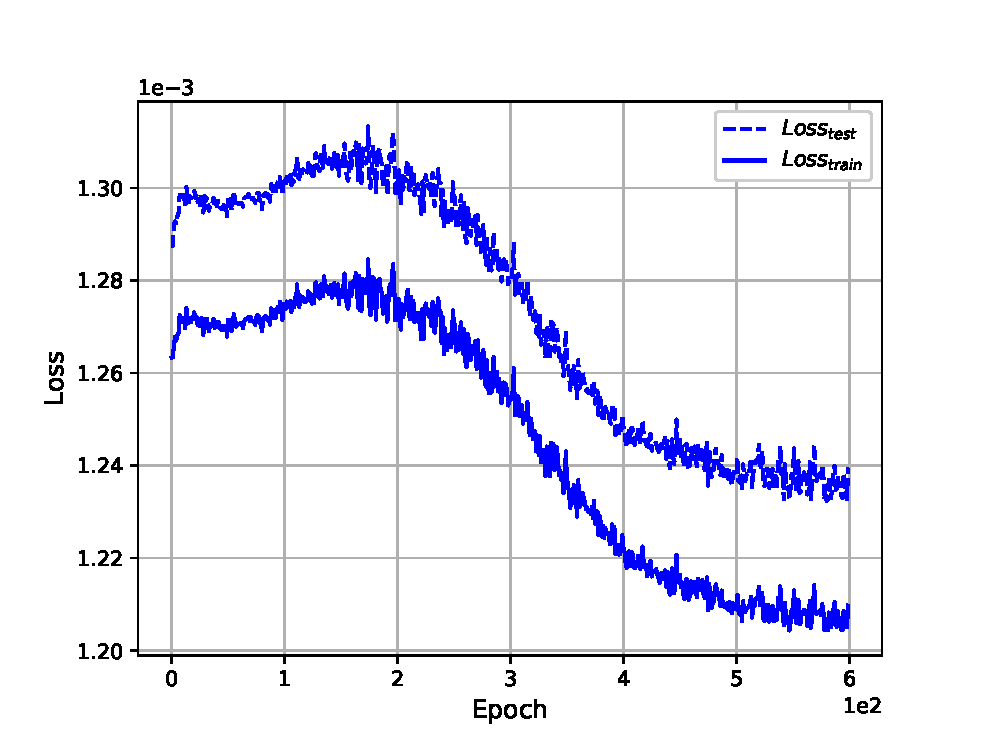
\includegraphics[width=\textwidth]{highdrop_losses}
        \caption{}
        \label{fig:dropout:high}
    \end{subfigure}
    \caption[Performance of the classifier for different dropout percentages]{Comparison of usual loss behaviour and loss behaviour including high dropout. Figure~\subref{fig:dropout:low} shows the losses for a dropout of \num{0.01}. Figure~\subref{fig:dropout:high} shows the losses for a dropout of \num{0.8}}
	\label{fig:simple_dropout}
\end{figure}


\subsection{Batch normalisation}

Batch normalisation was added to every deep layer and it had no significant effects on the output. Either the model does not develop any overly dominant features or dropout already does a sufficient job of normalisation. The extra layers were discarded for the classifying network to avoid an increase in computational time.
